\documentclass{amsart}

\usepackage[english]{babel}
\usepackage{csquotes}
\usepackage[sortcites=true, sorting=nyt, backend=biber]{biblatex}
\usepackage[colorlinks=true,
pdfstartview=FitV, linkcolor=blue, citecolor=olive,
urlcolor=cyan]{hyperref}
\usepackage{xcolor, soul} %Package to insert links, citations, etc.
\usepackage[english]{babel}
\usepackage{csquotes}
\usepackage{amsmath, amsthm, amssymb, mathtools}
\usepackage{graphicx} % Required for inserting images
\usepackage{geometry}
\usepackage{multicol}
\usepackage{tabularx}
\usepackage{changepage}
\usepackage[T1]{fontenc}
\usepackage{tikz, pgfplots, tikz-3dplot}
\usepackage{listings} % Used for inserting code snippets
\usepackage{comment}
\usepackage{setspace}
\usepackage{todonotes}
\usepackage{tcolorbox} % used for drawing boxes around paragraphs so that notes are easier to identify

\usepackage{enumitem}
\usepackage{listings} % Used for including code snippets
\usepackage{subcaption}

\geometry{letterpaper, portrait, margin=2in}%1in}

\graphicspath{{Images/}}

\usetikzlibrary{external}
\tikzexternalize[prefix=tikz/]

% This makes todonotes work with tikz external
\makeatletter
\renewcommand{\todo}[2][]{\tikzexternaldisable\@todo[#1]{#2}\tikzexternalenable}
\makeatother



\definecolor{myorange}{HTML}{ff7f00} % Defines the color of the box around text for tcolorbox
\definecolor{myblue}{HTML}{46b8ff} % Defines a blue color for notes that I make
\definecolor{darkgreen}{HTML}{008000} % Defines a dark green for lines

\newcommand{\mytodo}[2][]{\todo[color=myblue, #1]{#2}} % Makes a custom todo box for notes that I make vs notes Giuseppe makes.

%https://osl.ugr.es/CTAN/macros/latex/contrib/tcolorbox/tcolorbox.pdf
\tcbuselibrary{breakable}
\tcbset{%any default parameters
	width=0.7\textwidth,
	halign=justify,
	center,
	breakable,
	colback=myorange    
}

% This controls how the code snippets are typset
\lstset{
	basicstyle=\ttfamily,
	columns=fullflexible,
	frame=single,
	breaklines=true,
	postbreak=\mbox{\textcolor{red}{$\hookrightarrow$}}\space
}

\lstset{language=Octave}


\newtheorem{theorem}{Theorem}[section]
\newtheorem{lemma}[theorem]{Lemma}

\theoremstyle{definition}
\newtheorem{definition}{Definition}[section]
\newtheorem*{example*}{Example}
\newtheorem{example}{Example}[section]


\theoremstyle{remark}
\newtheorem{remark}{Remark}

\newlist{eqlist}{enumerate}{2}
\setlist[eqlist]{label=(\roman*), before=\raggedright}

% Nice way to make notes for myself
\newcommand{\William}[1]{\textcolor{red}{[William] #1}}

% Some nice math macros
\newcommand{\set}[1]{\left\{#1\right\}}
\newcommand*\diff{\mathop{}\!\mathrm{d}} % Changes the font of the differential d when writing dx or similar
\renewcommand{\st}{\colon} % renews the st command that is usually provided by soul to strike through
\newcommand{\N}{\mathbb{N}}
\newcommand{\R}{\mathbb{R}}
\newcommand{\Z}{\mathbb{Z}}
\newcommand{\Q}{\mathbb{Q}}
\newcommand{\RP}{\mathbb{RP}}
\newcommand{\Hyp}{\mathbb{H}}
\newcommand{\T}{\mathcal{T}}
\newcommand{\PSL}[2]{\mathsf{PSL}_{#1}\left(#2\right)}
\newcommand{\SL}[2]{\mathsf{SL}_{#1}\left(#2\right)}

\newcommand{\derof}[1]{\dot{#1}}
\newcommand{\der}{\mathsf{d}}
\newcommand{\crossratio}[1]{\operatorname{CR}\left[#1\right]}

\newcommand{\metricd}{\operatorname{d}}
\newcommand{\CR}[1]{\operatorname{CR}\left[#1\right]}
\newcommand{\bound}[1]{\partial #1}
\newcommand{\hvec}[2]{\begin{bmatrix} #1 \\ #2 \end{bmatrix}}

% Makes a todo list environment to make nice todo lists for things that would need to be shown
\newlist{todolist}{itemize}{2}
\setlist[todolist]{label=$\square$}

\newcommand{\inquotes}[1]{``#1''}

\newcommand{\close}[1]{\overline{#1}}

\newcommand{\wrt}{\text{w.r.t. }}
\newcommand{\projof}[1]{\pi\left(#1\right)}
\newcommand{\proj}{\pi}

% Used to make the bar to make the notation for a restricted domain look nicer
\newcommand{\littletaller}{\mathchoice{\vphantom{\big|}}{}{}{}}

% Makes a command to automatically created the notation for a restricted domain
\newcommand\restrict[2]{
	{% we make the whole thing an ordinary symbol
		\left.\kern-\nulldelimiterspace % automatically resize the bar with \right
		#1 % the function
		\littletaller % pretend it's a little taller at normal size
		\right|_{#2} % this is the delimiter
	}
}

%\frenchspacing
%\doublespacing

\newenvironment{summary}{
	\hfill \break 
	\begin{center}
		\textbf{Summary:}
	\end{center}
	\begin{adjustwidth}{0.5in}{0.5in}
		
	
}{
\end{adjustwidth}
\bigskip
}

\usetikzlibrary{arrows.meta}
\usetikzlibrary{shapes.geometric}
\usetikzlibrary{calc}
\usetikzlibrary{decorations.pathreplacing,shapes.misc}
\usetikzlibrary{intersections}
\usepgfplotslibrary{fillbetween}
\usepgfplotslibrary{colormaps}

\pgfplotsset{
	compat=1.18,
	colormap={mycolormap}{color=(lightgray) color=(white) color=(lightgray)}
}

\tikzset{
	convexset/.style = {line width = 0.75 pt, fill = white},
	ext/.style = {circle, inner sep=0pt, minimum size=2pt, fill=black},
	segment/.style = {line width = 0.75 pt}
}


% -- Tikz Pictures --

\tikzset{
	pics/torus/.style n args={3}{
		code = {
			\providecolor{pgffillcolor}{rgb}{1,1,1}
			\begin{scope}[
				yscale=cos(#3),
				outer torus/.style = {draw,line width/.expanded={\the\dimexpr2\pgflinewidth+#2*2},line join=round},
				inner torus/.style = {draw=pgffillcolor,line width={#2*2}}
				]
				\draw[outer torus] circle(#1);\draw[inner torus] circle(#1);
				\draw[outer torus] (180:#1) arc (180:360:#1);\draw[inner torus,line cap=round] (180:#1) arc (180:360:#1);
			\end{scope}
		}
	}
}

% --- End of Tikz Pictures ---


% -- Tikz Functions --

\tikzset{%
	add/.style args={#1 and #2}{
		to path={%
			($(\tikztostart)!-#1!(\tikztotarget)$)--($(\tikztotarget)!-#2!(\tikztostart)$)%
			\tikztonodes},add/.default={.2 and .2}}
} 

% https://tex.stackexchange.com/questions/86897/recover-scaling-factor-in-tikz
\newcommand*\getscale[1]{%
	\begingroup
	\pgfgettransformentries{\scaleA}{\scaleB}{\scaleC}{\scaleD}{\whatevs}{\whatevs}%
	\pgfmathsetmacro{#1}{sqrt(abs(\scaleA*\scaleD-\scaleB*\scaleC))}%
	\expandafter
	\endgroup
	\expandafter\def\expandafter#1\expandafter{#1}%
}


% -- End of Tikz Functions --
\addbibresource{thesis.bib}

\title{Visualizing the Manhattan Curve:\\Thesis Prospectus}
\author{William Clampitt}
\date{June 2, 2025}

\begin{document}
	\maketitle
	The goal of this project is to write a computer program to estimate the graph of the Manhattan curve of two convex real projective structures on the thrice-punctured sphere.
	
	\section{Topology Review}
	
	The first thing that we will want to review are some topology definitions that are relevant to this project. 
	
	\subsection{Definitions Review}
	
	\begin{definition}[Topological Space]
		A \emph{topological space} $X$ is a set together with a collection $\T$ of subsets of $X$ where $\T$ contains the sets $X$, $\varnothing$, and is closed under finite intersections and arbitrary unions. The elements of $\T$ are called open sets.
	\end{definition}
	
	\begin{definition}[$d$-manifold]
		Let $d\in \Z_{\geq 0}$. A \emph{$d$-manifold} is topological space that is second countable, Hausdorff, and locally Euclidean of dimension $d$.
	\end{definition}

	\begin{definition}[Locally Euclidean of Dimension $d$]
		A topological space $M$ is \emph{locally Euclidean of dimension $d$} if every point of $M$ is contained in an open set in $M$ that is homeomorphic to an open subset of $\R^d$.
	\end{definition}
	
	\begin{figure}[h]
		\centering
		\begin{subfigure}{0.3\textwidth}
			\centering
			\resizebox{2cm}{!}{
				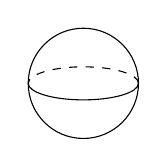
\begin{tikzpicture}[scale=.35,anchor=center]
					\draw (0,0) circle (2cm);
					\draw (-2,0) arc (180:360:2 and 0.6);
					\draw[dashed] (2,0) arc (0:180:2 and 0.6);
				\end{tikzpicture}
			}
			\caption{Sphere}
			\label{fig:example_sphere}
		\end{subfigure}
		\hfill
		\begin{subfigure}{0.3\textwidth}
			\centering
			\resizebox{2cm}{!}{
				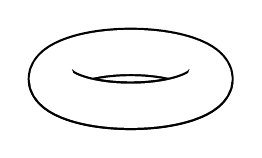
\begin{tikzpicture}[scale=.8,thick,anchor=center]
					\pic{torus={1cm}{2.8mm}{70}};
				\end{tikzpicture}
			}
			\caption{Torus}
			\label{fig:example_torus}
		\end{subfigure}
		\hfill
		\begin{subfigure}{0.3\textwidth}
			\centering
			\resizebox{2cm}{!}{
				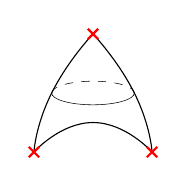
\begin{tikzpicture}[scale=.75,anchor=center]
					\draw[thin] plot[smooth,tension=1] coordinates {(-1,0) (-0.7,1) (0,2)};
					\draw[thin] plot[smooth,tension=1] coordinates {(1,0) (0.7,1) (0,2)};
					\draw[thin] plot[smooth,tension=1] coordinates {(-1,0) (0,.5) (1,0)};
					\node[cross out,draw,red, thick,scale=0.5] at (-1,0) {};
					\node[cross out,draw,red, thick,scale=0.5] at (1,0) {};
					\node[cross out,draw,red, thick,scale=0.5] at (0,2) {};
					\draw[very thin] (-.7,1) arc (180:360:.7 and .2);
					\draw[very thin, dashed] (-.7,1) arc (180:0:.7 and .2);
				\end{tikzpicture}
			}
			\caption{$S_{0,3}$}
			\label{fig:example_thice_punctured_sphere}
		\end{subfigure}
	\end{figure}
	
	Some examples of $2$-manifolds, or surfaces, are a sphere (Figure \ref{fig:example_sphere}) and a torus (Figure \ref{fig:example_torus}). Two other examples which will be the main players in this project are the sphere with three punctures, $S_{0,3}$ (Figure \ref{fig:example_thice_punctured_sphere}), and the set of lines passing through the origin in $\R^3$, denoted $\RP^2$. The topology on $S_{0,3}$ is the same as the topology on the unpunctured sphere and the basis for the topology on $\RP^2$ can be thought of as the cone around a fixed line $\ell$ through the origin in $\R^3$ that is formed by lines that differ from $\ell$ by at most a fixed, nonzero angle.
	
	\subsection{Alternate View of $\RP^2$}
	
	The definition of $\RP^2$ given in the previous section, however, is not very intuitive to visualize. In this section, an alternate way to view $\RP^2$ is given. Before we can discuss this alternate view, we will first define a few terms.
	
	\begin{definition}
		\label{def:affine_plane}
		A \emph{plane} in $\R^3$ is a $2$-dimensional vector subspace of $\R^3$. An \emph{affine plane} $A$ is a translate of a plane $P$ by a nonzero vector $v$ that is not in $P$.
	\end{definition}
	
	\begin{figure}[h]
		\begin{center}
			\tdplotsetmaincoords{70}{110}
			\begin{tikzpicture}[scale=2,tdplot_main_coords]
				\def\x{1.5}
				\filldraw[draw=blue,fill=blue!20]          
				(-1,-1,0)
				-- (1,-1,0)
				-- (1,1,0)
				-- (-1,1,0)
				-- cycle;
				
				\filldraw[draw=red,fill=red!20]          
				(-.5,-.5,1)
				-- (1.5,-.5,1)
				-- (1.5,1.5,1)
				-- (-.5,1.5,1)
				-- cycle;
				
				\draw[black, -Stealth, circle] (0,0,0) -- (.5,.5,1) node[anchor=north east]{$v$};
				\filldraw[black] (.5,.5,1) circle(.25pt) node[above right] {};
				\draw[thick,-Stealth] (0,0,0) -- (\x,0,0) node[anchor=north east]{$x$};
				\draw[thick,-Stealth] (0,0,0) -- (0,\x,0) node[anchor=north east]{$y$};
				\draw[thick,-Stealth] (0,0,0) -- (0,0,\x) node[anchor=north east]{$z$};
				\draw (-.5, 1.5, 1) node[above right]{$A$};
				\draw (-1, 1, 0) node[above right]{$P$};
			\end{tikzpicture}	
		\end{center}
		\caption{Plane $P$ through the origin in $\R^3$ with affine plane $A$.}
		\label{fig:affine_plane}
	\end{figure}
	
	\begin{lemma}
		\label{lem:RP2}
		Let $P$ be a plane passing through the origin in $\R^3$ and let $A$ be an affine plane which is a translate of $P$ by a nonzero vector $v$ not in $P$. Then,
		\begin{equation*}
			\RP^2 \cong A \sqcup \projof{P}
		\end{equation*}
		where $\projof{P}$ is the set of lines through the origin in $\R^3$ contained in $P$.
	\end{lemma}
	
	With these definitions, combined with Lemma \ref{lem:RP2}, we can visualize $\RP^2$ as the disjoint union of the projection of the plane $P$ through the origin in $\R^3$ and the affine plane $A$. We can do this mapping because a line $\ell$ through the origin in $\R^3$ is either fully contained in the plane $P$, or it exits the plane. In the first case, if $\ell$ is contained in $P$, then $\ell$ gets mapped to $\projof{P}$. In the second case, where $\ell$ is not fully contained within $P$, $\ell$ will intersect the affine plane $A$ at exactly one point, so $\ell$ gets mapped to this unique point in $A$.
	
	\section{Hyperbolic Structures}
	
	\subsection{The Upper Half Plane}
	
	The Upper Half Plane model of the hyperbolic plane consists of the upper half plane of $\R^2$, combined with the hyperbolic metric (Definition \ref{def:hyperbolic_plane}).
	
	\begin{definition}
		\label{def:hyperbolic_plane}
		The \emph{hyperbolic plane} $\Hyp^2$ is the metric space
		\begin{equation*}
			\Hyp^2 = \set{(x,y) \in \R^2 \colon y > 0} \qquad \metricd(u,v) = \inf_{u \to v} \int_0^1 \frac{\sqrt{\derof{x}(t)^2 + \derof{y}(t)^2}}{y(t)} \der{t}
		\end{equation*}
	\end{definition}
	
	\begin{figure}[h]
		\centering
		\begin{tikzpicture}[scale=.7]
			\begin{axis}[
				axis lines=middle,
				x axis line style={Stealth-Stealth, very thick},
				y axis line style={-{Stealth},very thick},
				xmin=-1.5, xmax=1.5, ymin=0, ymax=2.5,
				xlabel style={at={(axis description cs:1.04,0.04)},anchor=north},
				ylabel style={at={(axis description cs:0.45,1.04)},anchor=north},
				xlabel=$x$,
				ylabel=$y$,
				xticklabel=\empty,
				yticklabel=\empty,
				xtick=\empty,
				ytick=\empty]
				\addplot[domain=-.75:1.25,samples=400,blue,thick]{sqrt(1-(x-.25)^2)};
				\addplot+[only marks,mark=*,mark options={fill=black,black}, nodes near coords={$u$}] coordinates {(.3, 0.9987)};
				\addplot+[only marks,mark=*,mark options={fill=black,black}, nodes near coords={$v$}] coordinates {(1, 0.6614)};
			\end{axis}
		\end{tikzpicture}
		\caption{The Upper Half Plane model of $\Hyp_2$}
		\label{fig:upper_half_plane}
	\end{figure}
	
	While the top part of the hyperbolic metric looks similar to the Euclidean metric, dividing, because of the $y(t)$ in the denominator, things that look very close together near the $x$-axis are actually very far apart. Using this metric, the shortest path between two points $u,v \in \Hyp^2$ corresponds to the arc length of the portion of a semicircle, whose ends are perpendicular with the $x$-axis, that connects the points $u$ and $v$.
	
	\subsection{A Hyperbolic Structure on a Surface}
	
	We can now introduce a hyperbolic structure on a surface. Because a surface is a $2$-manifold, every point on a surface $S$ has a neighborhood around it that is homeomorphic to $\R^2$. Since $\Hyp^2$ is a subset of $\R^2$, but with a different metric, for every point $p \in S$, we can find a local homeomorphism from a neighborhood of $p$ to $\Hyp^2$. The collection $G$ of all of local homeomorphisms from $S$ to $\Hyp^2$ is called an \emph{atlas}.
	
	Let $\alpha$ and $\beta$ be distinct points in $S$ and let $U_\alpha$ and $U_\beta$ be open neighborhoods of $\alpha$ and $\beta$, respectively, that are homeomorphic to $\Hyp^2$. Now, let
	\begin{equation*}
		\begin{split}
			\varphi_\alpha & \colon U_\alpha \to V_\alpha \\
			\varphi_\beta & \colon U_\beta \to V_\beta
		\end{split}
	\end{equation*}
	
	be homeomorphisms to $\Hyp^2$. The neighborhoods $U_\alpha, U_\beta \subseteq S$ and $V_\alpha, V_\beta \subseteq \Hyp^2$ are shown in Figures \ref{fig:neighborhoods_in_S} and \ref{fig:neighborhoods_in_H2}, respectively.
	
	\begin{figure}[h]
		\begin{subfigure}{.45\textwidth}
			\includegraphics[width=\textwidth]{neighborhoods_in_S}	
			\caption{Neighborhoods in $S$}
			\label{fig:neighborhoods_in_S}
		\end{subfigure}
		\hfill
		\begin{subfigure}{.45\textwidth}
			\includegraphics[width=\textwidth]{neighborhoods_in_H2}
			\caption{Image of $\varphi_\alpha$ and $\varphi_\beta$ in $\Hyp^2$}
			\label{fig:neighborhoods_in_H2}
		\end{subfigure}
		\caption{Local homeomorphism from $S$ to $\Hyp^2$}
		\label{fig:local_homeomorphisms}
	\end{figure}
	
	
	We then can look at the map
	\begin{equation*}
		\varphi_\beta \circ \varphi_\alpha^{-1} \colon \varphi_\alpha(U_\alpha \cap U_\beta) \to \varphi_\beta(U_\alpha \cap U_\beta).
	\end{equation*}
	
	This map is referred to as a \emph{change of charts}. If the restriction 
	\begin{equation*}
		\restrict{\varphi_\beta \circ \varphi_\alpha^{-1}}{\varphi_\alpha(U_\alpha) \cap \varphi_\beta(U_\beta)}
	\end{equation*} 
	
	is an isometry for all $\alpha, \beta \in S$, then the atlas $G$, equipped with the metric space $\Hyp^2$, is a geometric structure on $S$. In general, this process can be done with any $d$-manifold and appropriate metric space.
	
	
	\subsection{Fundamental Groups}
	\label{sec:fundamental_groups}
	
	Now, we will discuss the idea of the fundamental group on a surface and will later discuss a geometric way to represent the elements of the fundamental group.
	
	\begin{definition}
		Let $S$ be a path-connected a surface. For any point $p\in S$ the \emph{fundamental group} of $S$ is the set of equivalence classes (under homotopy) of the loops on $S$ based at $p$ with the concatenation operation. This group is denoted $\pi_1(S)$.
	\end{definition}
	
	We will see an example later on that a hyperbolic structure on a surface gives us a way to associate each element of the fundamental group with an element in $\PSL{2}{\R}$.
	
	\subsection{The Hyperbolic Structure on $\mathbf{ S_{0,3} }$}
	
	In general, there are many different hyperbolic structures that could be placed on a surface. However, $S_{0,3}$ has only one hyperbolic structure, as we now explain.
	
	\begin{lemma}
		\label{lem:triple_invertible_matrix}
		For any triple $(x,y,z)$ of pairwise distinct points in $\RP^1$, there exists a $2\times2$ invertible matrix sending
		\begin{equation*}
			\begin{split}
				x & \to \text{ a multiple of } \hvec{-1}{1} \\
				y & \to \text{ a multiple of } \hvec{0}{1} \\
				z & \to \text{ a multiple of } \hvec{1}{0}.
			\end{split}
		\end{equation*}
	\end{lemma} 
	
	\begin{proof}
		Let $x,y,z \in \RP^1$ be pairwise distinct points, $a,b,c,d \in \R$,
		\begin{equation*}
			A = 
			\begin{bmatrix}
				a & b \\
				c & d
			\end{bmatrix},
		\end{equation*}
		\begin{equation*}
			x = \hvec{x_1}{x_2},\quad y = \hvec{y_1}{y_2},\text{ and }\quad z = \hvec{z_1}{z_2}.
		\end{equation*}
		
		Because $x,y,$ and $z$ are pairwise distinct and only defined up to scaling, we can let $x_2 = y_2 = 1$ and $z_1 = 1$.
		
		Now we have,
		\begin{align*}
			Ax &= 
			\begin{bmatrix}
				a & b \\
				c & d
			\end{bmatrix} 
			\hvec{x_1}{1}
			= \hvec{x_1a + b}{x_1c + d} \\
			Ay &=
			\begin{bmatrix}
				a & b \\
				c & d
			\end{bmatrix}
			\hvec{y_1}{1}
			= \hvec{y_1a + b}{y_1c + d} \\
			Az &=
			\begin{bmatrix}
				a & b \\
				c & d
			\end{bmatrix}
			\hvec{1}{z_2}
			= \hvec{a + z_2b}{c + z_2d}.
		\end{align*}
		
		Since we want $Ax$ to be a multiple of $\hvec{-1}{1}$, $Ay$ to be a multiple of $\hvec{0}{1}$, and $Az$ to be a multiple of $\hvec{1}{0}$,
		\begin{align*}
			Ax &= \hvec{x_1a + b}{x_1c + d} &\implies& -(x_1c + d) = (x_1a + b) \\
			Ay &= \hvec{y_1a + b}{y_c + d} &\implies& y_1a + b = 0 \\
			Az &= \hvec{a + z_2b}{c + z_2d} &\implies& c + z_2d = 0
		\end{align*}
		
		Doing some algebra, we can solve for $a,b$, and $c$ to get
		\begin{align*}
			a &= \frac{1 - x_1z_2}{y_1 - x_1}d \\
			b &= -y_1 \left( \frac{1 - x_1z_2}{y_1 - x_1}\right) d \\
			c &= -z_2 d \\
			d &= d
		\end{align*}		
		
		Because $x$ and $y$ are pairwise distinct and $x_2 = y_2$, $x_1 \neq y_1$, therefore $y_1 - x_1 \neq 0$. 
		
		Since we want the matrix $A$ to be invertible, $\det(A)$ needs to be nonzero.
		
		\begin{equation*}
			\det(A) = d^2\frac{(1 - x_1z_2)(1-z_2y_1)}{y_1-x_1}
		\end{equation*}
		
		Suppose $1-x_1z_2 = 0$. This would imply that $z_2 = \frac{1}{x_1}$. Then 
		\begin{equation*}
			x = \hvec{x_1}{1} = x_1 \hvec{1}{\frac{1}{x}} = x_1 z.
		\end{equation*}
		
		This contradicts $x$ and $z$ being pairwise distinct points in $\RP^1$. Therefore $1-x_1z_2 \neq 0$. By similar reasoning, $1-z_2y_1 \neq 0$. Therefore, $\det(A) = 0$ only when $d=0$.
		Therefore, $A$ is invertible when $d\neq 0$, so we have found infinitely many $2 \times 2$ invertible matrices that fit our desired criteria.
	\end{proof}
	
	\bigskip
	
	\begin{theorem}
		There is only one hyperbolic structure on $S_{0,3}$.
	\end{theorem}
	
	\bigskip

	\begin{proof}
		We can lift the the front of $S_{0,3}$ to the universal cover of $S_{0,3}$ which gives us a triangle in $\Hyp^2$ with verticies at infinity, called $p_{rg}$, $p_{gb}$, and $p_{rb}$ (Figure \ref{fig:hyperbolic_structure_S03}). Since $\bound{\Hyp^2} \cong \RP^1$, we have three pairwise distinct points in $\RP^1$, we can use Lemma \ref{lem:triple_invertible_matrix} to \inquotes{normalize} these points to the vectors
		\begin{equation*}
			p_{rg} = \hvec{-1}{1} \quad p_{gb} = \hvec{0}{1} \quad p_{rb} = \hvec{1}{0}.
		\end{equation*}
		
		The back triangle lifts to points $\hvec{x}{1}, \hvec{0}{1},$ and $\hvec{1}{0}$ (Shown in yellow on Figure \ref{fig:S03_in_H2}).
		
			\begin{figure}[h!]
			\begin{subfigure}{.45\textwidth}
				\centering
				\resizebox{\textwidth}{!}{
					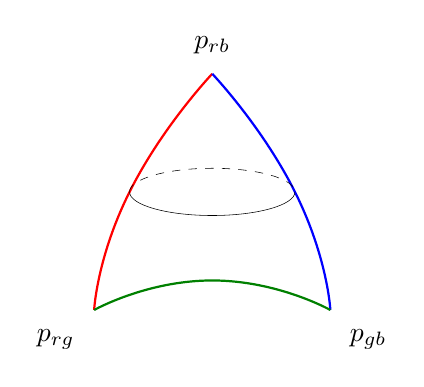
\begin{tikzpicture}[scale=1.5,baseline=(current bounding box.center)]
						\draw[thick,red] plot[smooth,tension=1] coordinates {(-1,0) (-0.7,1) (0,2)};
						\draw[thick,blue] plot[smooth,tension=1] coordinates {(1,0) (0.7,1) (0,2)};
						\draw[thick,darkgreen] plot[smooth,tension=1] coordinates {(-1,0) (0,.25) (1,0)};
						\draw[very thin] (-.7,1) arc (180:360:.7 and .2);
						\draw[very thin, dashed] (-.7,1) arc (180:0:.7 and .2);
						\node[label=below left:{$p_{rg}$}] at (-1,0) {};
						\node[label=above:{$p_{rb}$}] at (0,2) {};
						\node[label=below right:{$p_{gb}$}] at (1,0) {};
					\end{tikzpicture}
				}
				\caption{$S_{0,3}$ with colored edges}
				\label{fig:S03_colored_edges}
			\end{subfigure}
			\hfill
			\begin{subfigure}{.45\textwidth}
				\resizebox{\textwidth}{!}{
					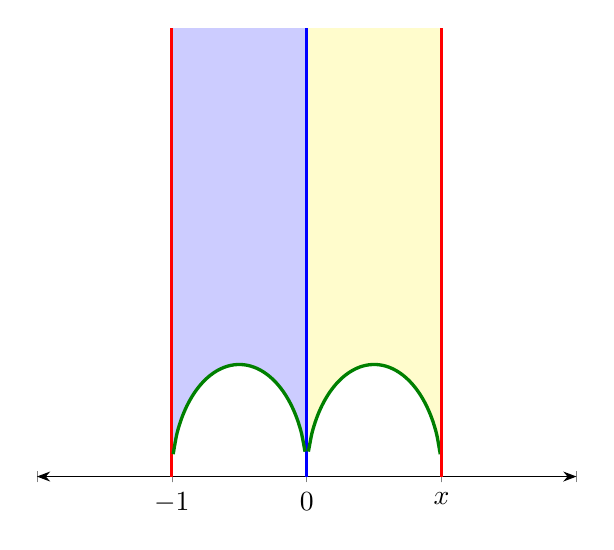
\begin{tikzpicture}[scale=1,baseline=(current bounding box.center)]
						\begin{axis}[
							axis lines=middle,
							x axis line style={Stealth-Stealth, thin},
							xmin=-2, xmax=2, ymin=0, ymax=2,
							xticklabel=\empty,
							yticklabel=\empty,
							extra x ticks={-1,0,1},
							extra x tick labels={$-1$,0,$x$},
							ytick=\empty]
							\draw[red,very thick] (-1,0) -- (-1,2);
							\draw[blue,very thick] (0,0) -- (0,2);		
							\addplot+[smooth,samples=400,very thick,no marks,darkgreen,name path=A] {sqrt(.25-(x+.5)^2)}; 
							\addplot+[draw=none,no marks,name path=B] {2};     
							\addplot+[blue!20] fill between[of=A and B,soft clip={domain=-1:0}];
							\addplot+[smooth,samples=400,very thick,no marks,darkgreen,name path=C] {sqrt(.25-(x-.5)^2)}; 
							\draw[red,very thick] (1,0) -- (1,2);
							\addplot+[draw=none,no marks,name path=D] {2};     
							\addplot+[yellow!20] fill between[of=C and D,soft clip={domain=0:1}];
							\draw[red,very thick] (1,0) -- (1,2);
						\end{axis}
					\end{tikzpicture}
				}
				\caption{$S_{0,3}$ represented in $\Hyp^2$}
				\label{fig:S03_in_H2}
			\end{subfigure}
			\caption{Color-coded edges to show the image of corresponding punctures in $\Hyp^2$.}
			\label{fig:hyperbolic_structure_S03}
		\end{figure}
		
		\begin{comment}
			\hl{the color-coded explanation should be in the caption of the figure. Say "In the math, I call these $p_{rg}$, $p_{gb}$, etc. and the back triangle lifts to points ... and $\hvec{x}{1}$ for some $x>1$. We wish to prove that $x=1$.}	
		\end{comment}
		
		Our first goal is to find a matrix $P_1 \in \PSL{2}{\R}$ that represents the loop on the surface $S_{0,3}$ that goes around the puncture $p_{rb}$. This means that we want $P_1$ to send
		\begin{align*}
			\hvec{-1}{1} & \to \text{ a multiple of } \hvec{x}{1} \text{ and }\\
			\hvec{1}{0} & \to \text{ a multiple of } \hvec{1}{0}.
		\end{align*}
		
		We can let 
		\begin{equation*}
			P_1 = 
			\begin{bmatrix}
				a_1 & a_2 \\
				a_3 & a_4
			\end{bmatrix}
		\end{equation*}
		
		and see that
		\begin{align*}
			\begin{bmatrix}
				a_1 & a_2 \\
				a_3 & a_4
			\end{bmatrix}
			\hvec{1}{0} &= \hvec{a_1}{a_3}.	
		\end{align*}
		
		Since we want $P_1 p_{rb}$ to be multiple of $\hvec{1}{0}$, this implies that $a_3 = 0$. Because $P_1 \in \PSL{2}{\R}$, $\det(P_1) = \pm 1$. Suppose $\det(P_1) = 1$. Then,
		\begin{equation*}
			\det\left(
			\begin{bmatrix}
				a_1 & a_2 \\
				0 & a_4
			\end{bmatrix}
			\right) = a_1a_4 = 1
		\end{equation*}
		
		which implies that $a_4 = \frac{1}{a_1}$. Now, we can look at
		\begin{equation*}
			\begin{bmatrix}
				a_1 & a_2 \\
				0 & \frac{1}{a_1}
			\end{bmatrix}
			\hvec{-1}{1} = \hvec{-a_1 + a_2}{\frac{1}{a_1}}.
		\end{equation*}
		
		Since we want $P_1 p_{rg}$ to be a multiple of $\hvec{x}{1}$, we get that $-a_1 + a_2 = \frac{1}{a_1}x$ which implies that $a_2 = a_{1} + \frac{1}{a_1}x$.
		
		Because we want $P_1$ to represent a loop around the puncture $p_{rb}$, we want the eigenvalues of $P_1$ to be either both $1$ or both $-1$. The characteristic equation of $P_1$ is
		\begin{equation*}
			( a_1 - \lambda)(\frac{1}{a_1} - \lambda) = 0
		\end{equation*}
		
		so $a_1 = \lambda$, $\frac{1}{a_1} = \lambda$, so we will let $a_1 = 1$. We then have the matrix
		\begin{equation*}
			P_1 = 
			\begin{bmatrix}
				1 & 1 + x \\
				0 & 1
			\end{bmatrix}.
		\end{equation*}
		
		To find the matrix $P_2$ that represents the loop around the puncture $p_{gb}$, we can do a similar calculation to find the matrix that sends 
		\begin{align*}
			\hvec{0}{1} & \to \text{ a multiple of } \hvec{0}{1} \text{ and }\\
			\hvec{-1}{1} & \to \text{ a multiple of } \hvec{x}{1}.
		\end{align*}
		
		When we do this, we end up with
		\begin{equation*}
			P_2 = 
			\begin{bmatrix}
				1 & 0 \\
				\frac{1 + x}{x} & 1
			\end{bmatrix}.
		\end{equation*}
		
		Finally, we want to find the matrix that represents the loop around the puncture $p_{rg}$. We can notice that this loop, which we will call $P_3$, is equivalent to $P_2 P_1^{-1}$. Because we want $P_3$ to represent a loop around a puncture, the eigenvalues of $P_3$ should be either both $1$ or both $-1$. If we solve for the eigenvalues, we end up with the characteristic polynomial
		\begin{equation*}
			\lambda^2 + \left(x + \frac{1}{x}\right)\lambda + 1 = (\lambda + x)\left(\lambda + \frac{1}{x}\right) = 0.
		\end{equation*}
		
		Since $\lambda = \pm 1$ and $x$ is nonnegative, we see that the only value that $x$ can be is $1$. Thus, the hyperbolic structure on $S_{0,3}$ is unique.
	\end{proof}
	
	
	%\mytodo[inline]{Fix the alignment of the pictures in Figure \ref{fig:hyperbolic_structure_S03}}
	
	\section{Convex Real Projective Structures}
	
	Although there is only one hyperbolic structure on $S_{0,3}$, that is not the only geometric structure that can placed on $S_{0,3}$. To discuss this, let's define some terms that will be relevant to the discussion.
	
	\begin{definition}
		An open set $\Omega \subseteq \RP^2$ is \emph{proper} if there exists a plane $P \subseteq \R^3$ passing through the origin such that $\close{\Omega} \cap \projof{P} = \varnothing$. A proper set $\Omega \subseteq \RP^2$ is \emph{convex} if, for any two points $x,y \in \Omega$, the line $l_{xy}$ passing though $x$ and $y$ intersects $\Omega$ in a connected segment. The proper, convex set $\Omega$ is \emph{strictly convex} if $\bound{\Omega}$ contains no straight line segments.
	\end{definition}
	
	\begin{figure}[h]
		\centering
		\begin{subfigure}{0.3\textwidth}
			\centering
			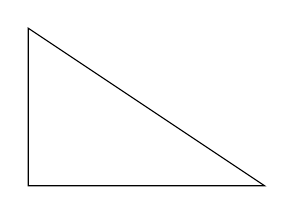
\begin{tikzpicture}[anchor=center]
				\draw (0,0) -- (3,0) -- (0,2) -- cycle;
			\end{tikzpicture}
			\caption{Triangle}
			\label{fig:triangle}
		\end{subfigure}
		\hfill
		\begin{subfigure}{0.3\textwidth}
			\centering
			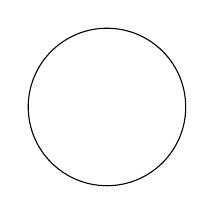
\begin{tikzpicture}[anchor=center]
				\draw (0,0) circle (1);
			\end{tikzpicture}
			\caption{Circle}
			\label{fig:circle}
		\end{subfigure}
		\hfill
		\begin{subfigure}{0.3\textwidth}
			\centering
			\includegraphics[width=\textwidth]{strictly_convex_set_from_paper}
			\caption{\cite{degerneration_of_Hilbert_metric} Numerical approximation of a strictly convex set}
			\label{fig:RP2_Structure}
		\end{subfigure}
	\end{figure}
	
	\begin{definition}
		Given a strictly convex set $\Omega$ in $\RP^2$, the \emph{Hilbert distance} between any two distinct points $a,b \in \Omega$ is given by
		\begin{equation*}
			\metricd(a,b) =  \frac{1}{2} \log \CR{x,a,b,y}
		\end{equation*}
	\end{definition}
	
	\begin{figure}[h]
		\begin{center}
			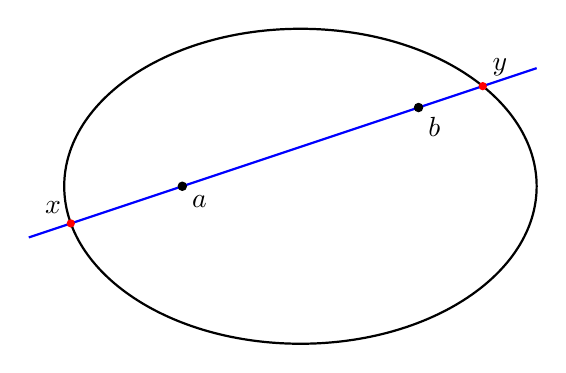
\begin{tikzpicture}
				\draw[thick,name path=line 1] (0,0) ellipse (3 and 2);
				\coordinate (a) at (-1.5,0);
				\coordinate (b) at (1.5,1);
				\node[below right] at (a) {$a$};
				\node[below right] at (b) {$b$};
				\draw[add= .65 and .5, blue, thick,name path=line 2] (a) to (b);
				\draw[fill=black] (a) circle (1.5pt);
				\draw[fill=black] (b) circle (1.5pt);
				\fill[red,name intersections={of=line 1 and line 2,total=\t}]
				\foreach \s in {1,...,\t}{(intersection-\s) circle (1.5pt)};
				\node[above left] at (intersection-2) {$x$};
				\node[above right] at (intersection-1) {$y$};
			\end{tikzpicture}	
		\end{center}
		\caption{The Hilbert distance in a convex $\RP^2$ structure}
		\label{fig:hilbert_distance}
	\end{figure}
	
	In a convex real projective structure, instead of using the atlas from $S_{0,3}$ to $\Hyp^2$, we can instead look at the local homeomorphims from $S_{0,3}$ to a strictly convex set $\Omega \subseteq \RP^2$. We can represent a loop on the surface of $S_{0,3}$ using the reflection matrices shown in \eqref{eq:reflection_matrices}. The parameter $T$ in \eqref{eq:reflection_matrices} determines the shape of $\Omega$. We can place the points where the punctures occur in $S_{0,3}$ at three basis vectors in $\R^3$. In the case of Figure \ref{fig:reflections_in_Omega}, the standard normal basis vectors in $\R^3$ were chosen.
	
	\begin{equation}
		R_{1,T} = 
		\begin{bmatrix}
			-1 & 0 & 0 \\
			2T & 1 & 0 \\
			\frac{2}{T} & 0 & 1
		\end{bmatrix}
		\ 
		R_{2,T} = 
		\begin{bmatrix}
			1 & \frac{2}{T} & 0 \\
			0 & -1 & 0 \\
			0 & 2T & 1
		\end{bmatrix}
		\ 
		R_{3,T} = 
		\begin{bmatrix}
			1 & 0 & 2T \\
			0 & 1 & \frac{2}{T} \\
			0 & 0 & -1
		\end{bmatrix}
		\label{eq:reflection_matrices}
	\end{equation}
	
	\begin{figure}[h]
		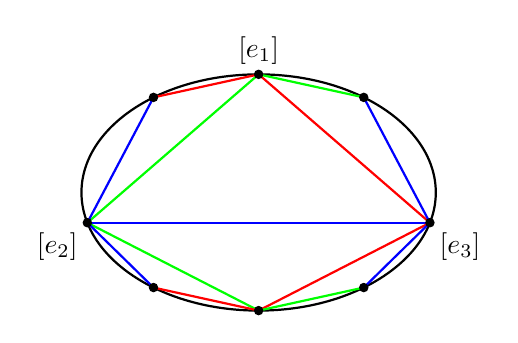
\begin{tikzpicture}[
			scale=1.5,
			R1_edge/.style={blue, thick},
			R2_edge/.style={red, thick},
			R3_edge/.style={green, thick}
			]
			\coordinate (e1) at (0,1);
			\coordinate (e2) at (-1.45,-0.25604);
			\coordinate (e3) at (1.45,-0.25604);
			\coordinate (R1e1) at (0,-1);
			\coordinate (R1R2e1) at (-.89,-0.80496);
			\coordinate (R1R3e1) at (.89,-0.80496);
			
			\coordinate (R2e2) at (.89,0.80496);
			\coordinate (R3e3) at (-.89,0.80496);
			
			\draw[thick] (0,0) ellipse (1.5cm and 1cm);
			\node[above] (pe1) at (e1) {$[e_1]$};
			\node[below left] (pe2) at (e2) {$[e_2]$};
			\node[below right] (pe3) at (e3) {$[e_3]$};
			
			\draw[R1_edge] (e2) -- (e3);
			\draw[R2_edge] (e1) -- (e3);
			\draw[R3_edge] (e1) -- (e2);
			
			\draw[R3_edge] (e2) -- (R1e1);
			\draw[R2_edge] (e3) -- (R1e1);
			
			\draw[R2_edge] (R1R2e1) -- (R1e1);
			\draw[R1_edge] (R1R2e1) -- (e2);
			\draw[R3_edge] (R1e1) -- (R1R3e1);
			\draw[R1_edge] (e3) -- (R1R3e1);
			
			\draw[R3_edge] (R2e2) -- (e1);
			\draw[R1_edge] (R2e2) -- (e3);
			
			\draw[R1_edge] (R3e3) -- (e2);
			\draw[R2_edge] (R3e3) -- (e1);
			
			\draw[fill=black,black] (e1) circle[radius=1pt];
			\draw[fill=black,black] (e3) circle[radius=1pt];
			\draw[fill=black,black] (e2) circle[radius=1pt];
			
			\draw[fill=black,black] (R1e1) circle[radius=1pt];
			\draw[fill=black,black] (R1R2e1) circle[radius=1pt];
			\draw[fill=black,black] (R1R3e1) circle[radius=1pt];
			
			\draw[fill=black,black] (R2e2) circle[radius=1pt];
			\draw[fill=black,black] (R3e3) circle[radius=1pt];
		\end{tikzpicture}
		\caption{Reflections of $S_{0,3}$ in $\Omega$}
		\label{fig:reflections_in_Omega}
	\end{figure}
	
	Using this method, we can place uncountably many convex real projective structures on $S_{0,3}$. When $T = 1$, there is an isometry between the convex real projective structure and the hyperbolic structure on $S_{0,3}$.
	
	\section{Hilbert Entropy}
	
	The representation of the elements in $\pi_1(S_{0,3})$ as a word in $\PSL{3}{\R}$ forms a group action on the set $\Omega$. We can then measure how \inquotes{chaotic} our convex real projective structure on $S_{0,3}$ is by measuring how far a group element moves a given point in $\Omega$. This is where the concept of entropy is useful.
	
	\begin{definition}
		Let $\Omega$ be a convex real projective structure on a surface $S$ and $p \in \Omega$ be a fixed point. The Hilbert \emph{entropy} is given by
		\begin{equation*}
			h_\Omega = \lim_{x \to \infty} \frac{1}{x} \log \#\set{\gamma \in \pi_1(S_{0,3}) \colon \metricd_\Omega(p,\rho_T(\gamma)p) \leq x}
		\end{equation*}
		\textbf{Note:} $\rho_T \colon \pi_1(S_{0,3}) \to \PSL{3}{\R}$	
	\end{definition}
	
	\section{The Manhattan Curve}
	
	Now that we have a way to measure the \inquotes{chaos} of a specific convex $\RP^2$ structure on $S_{0,3}$, it is useful to be able to compare the entropy of any two convex $\RP^2$ structures. 
	
	Let $a$ and $b$ be nonnegative real numbers such that $a_1 + a_2 = 1$. Then
	
	\begin{equation*}
		h_{a_1,a_2}^{T_1,T_2} = \lim_{x \to \infty} \frac{1}{x} \log \#\set{\gamma \in \pi_1(S_{0,3}) \colon a_1\metricd_1(p,\rho_1(\gamma)p) + a_2\metricd_{2}(p,\rho_2(\gamma)p) \leq x}
	\end{equation*}
	
	where $\rho_1$ and $\rho_2$ map an element in $\pi_1(S_{0,3})$ to a word made with the alphabet \eqref{eq:reflection_matrices} with parameter $T_1$ and $T_2$, respectively and $\metricd_1$ and $\metricd_2$ are the respective metrics in the spaces $\Omega_1$ and $\Omega_2$.

	\begin{figure}[h]
		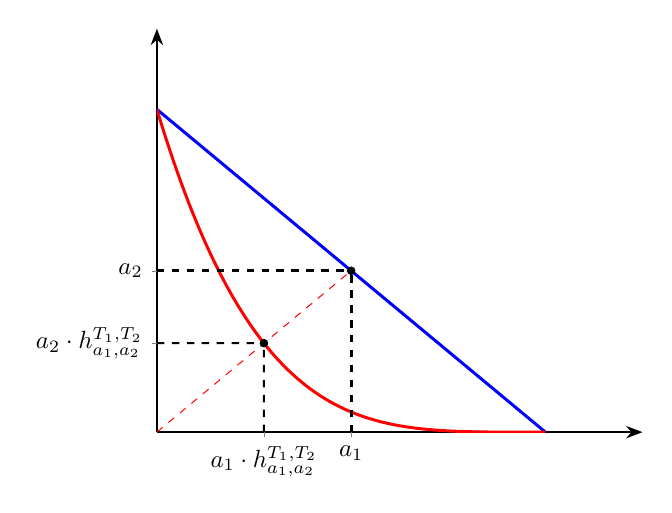
\begin{tikzpicture}[scale=.9]
			\newcommand{\pointa}{.5}
			\newcommand{\pointb}{.5}
			\newcommand{\ha}{0.27551}
			\newcommand{\hb}{0.27551}
			\begin{axis}[
				axis lines=middle,
				x axis line style={-{Stealth}, thick},
				y axis line style={-{Stealth},thick},
				xmin=0, xmax=1.25, ymin=0, ymax=1.25,
				xticklabel=\empty,
				yticklabel=\empty,
				ytick=\empty,
				xtick=\empty,
				extra x ticks={\ha,\pointa},
				extra x tick labels={$a_1 \cdot h_{a_1,a_2}^{T_1,T_2}$,$a_1$},
				extra y ticks={\hb,\pointb},
				extra y tick labels={$a_2 \cdot h_{a_1,a_2}^{T_1,T_2}$,$a_2$}
				]
				\addplot[domain=0:1,samples=5,blue,very thick]{-x+1};
				\addplot[smooth,domain=0:1,samples=100,red,very thick,name path=thecurve]{(x-1)^4};
				\coordinate (ab) at (\pointa,\pointb);
				\coordinate (hpoint) at (\ha,\hb);
				\draw[black,very thick,dashed] (\pointa,0) -- (ab);
				\draw[black,very thick,dashed] (0,\pointb) -- (ab);
				\draw[black,fill=black] (ab) circle (1.5pt);
				\draw[thin,red,dashed,name path=abline] (0,0) -- (ab);
				\fill[red,name intersections={of=abline and thecurve,total=\t}]
				\foreach \s in {1,...,\t}{(intersection-\s) circle (1.5pt)};
				\draw[black,fill=black] (intersection-1) circle (1.5pt);
				\draw[black,thick,dashed] (\ha,0) -- (intersection-1);
				\draw[black,thick,dashed] (0,\hb) -- (intersection-1);
			\end{axis}
		\end{tikzpicture}
		\caption{The Manhattan Curve}
		\label{fig:manhattan_curve}
	\end{figure}
	
	The Manhattan curve has very nice properties, such as being strictly convex and real analytic, which is very useful in fields such as dynamical systems.
	
	\section{Code to Estimate Entropy}
	
	The goal of this project is to write an Octave program that will graph the Manhattan curve when given two convex real projective structures on $S_{0,3}$.
	
	\subsection{Goals of the Code}
	
	The way that this program acomplishes this goal of plotting the Manhattan curve is by doing the following:
	\begin{enumerate}[label=\arabic*.]
		\item generate as many group elements as possible,
		\item store the singular values of each group element (the singular values are related to $\metricd_\Omega(p,\rho_T(\gamma)p)$),
		\item estimate the entropy for a given parameter $T$, and finally,
		\item graph the Manhattan curve given two convex real projective structures.
	\end{enumerate}
	
	\subsection{How the Code Works}
	
	Because we need to generate as many group elementss as possible, we leverage the inherent tree structure of the universal cover to create many elements in our group while avoiding duplicate elements. The program keeps track of the tree structure, then multiplies the appropriate matrices, \eqref{eq:reflection_matrices}, to create a word in $\PSL{2}{\R}$. These words and their singular values are then written to a file to be used in later calculations. 
	
	Once all the requested matrices are calulated, the program goes back and reads the files that contains the singular values and calculates the \inquotes{length} of a word using the formula $\ln\left(\frac{\sigma_3}{\sigma_1}\right)$, where $\sigma_3$ and $\sigma_1$ are the largest and smallest singular values, respectively. This resulting number is then grouped into an interval $[n,n+1)$, where $n \in \Z_{\geq 0}$. A tally is kept of how many group element's lengths fell into each interval. This creates a sequence of numbers whose limit will approach the entropy of our convex real projective structure.
	
	\subsection{Program Execution}
	
	In its current state, the program can calculate 4,194,302 group elements in just over 10.5 minutes. Due to the nature of these calculations, the time required to calculate the number of words that are $n$ verticies away from the root of the tree grows exponentially. 
	
	\section{Future Directions}
	
	Possible directions that this research could explore in the future are analyzing symmetries of the Manhattan curve, estimating the coordinates of the point where the slope of the tangent line of the Manhattan curve is equal to the slope of the secand line between the axes intercepts (this is a dynamical quantity called the \emph{correlation number}), or analyzing what happens to the Manhattan curve $\mathcal{M}(\rho_1,\rho_T)$ when $T$ gets very large. In addition to this, we can continue to generate more examples of these groups for differrent values of the parameter $T$, and different methods of optimizing the code could be explored so that we can generate even more group elements. One potential optimization method could be exploring different data structures that could more efficiently store the information about the generated matrices. Another potential optimization would be to implement some form of parallel processing which would allow us to calculate many more group elements simultaniously which would significantly increase the speed at which we can generate new group elements.
	\newpage
	\printbibliography
	
\end{document}